% ------------------------------------------------------------------------------
% TYPO3 CMS 8.0 - What's New (English Version)
%
% @author	Patrick Lobacher <patrick@lobacher.de> and Michael Schams <schams.net>
% @license	Creative Commons BY-NC-SA 3.0
% @link		http://typo3.org/download/release-notes/whats-new/
% @language	English
% ------------------------------------------------------------------------------
% LTXE-CHAPTER-UID:		d71b4b88-f79b2343-d2b356bf-452cef81
% LTXE-CHAPTER-NAME:	Backend User Interface
% ------------------------------------------------------------------------------

\section{Backend User Interface}
\begin{frame}[fragile]
	\frametitle{Backend User Interface}

	\begin{center}\huge{Chapter 1:}\end{center}
	\begin{center}\huge{\color{typo3darkgrey}\textbf{Backend User Interface}}\end{center}

\end{frame}

% ------------------------------------------------------------------------------
% LTXE-SLIDE-START
% LTXE-SLIDE-UID:		0ca78dc4-0ffa7d70-64f9a1d3-253878c0
% LTXE-SLIDE-ORIGIN:	d8599a04-11b4fa8c-9be5812a-715820e1 English
% LTXE-SLIDE-ORIGIN:	ef1d6d8c-0db67396-dedb5814-1767169f German
% LTXE-SLIDE-TITLE:		Recover pages recursively to top of rootline
% LTXE-SLIDE-REFERENCE:	!Feature-1835-RecoverPagesRecursivelyToTop.rst
% ------------------------------------------------------------------------------
\begin{frame}[fragile]
	\frametitle{Backend User Interface}
	\framesubtitle{Recover pages recursively to top of rootline}

	The Recycler supports the recursive recovery of deleted pages to the top of the rootline now.
	This feature is available for admin users only due to internal permission restrictions.

	\begin{figure}
		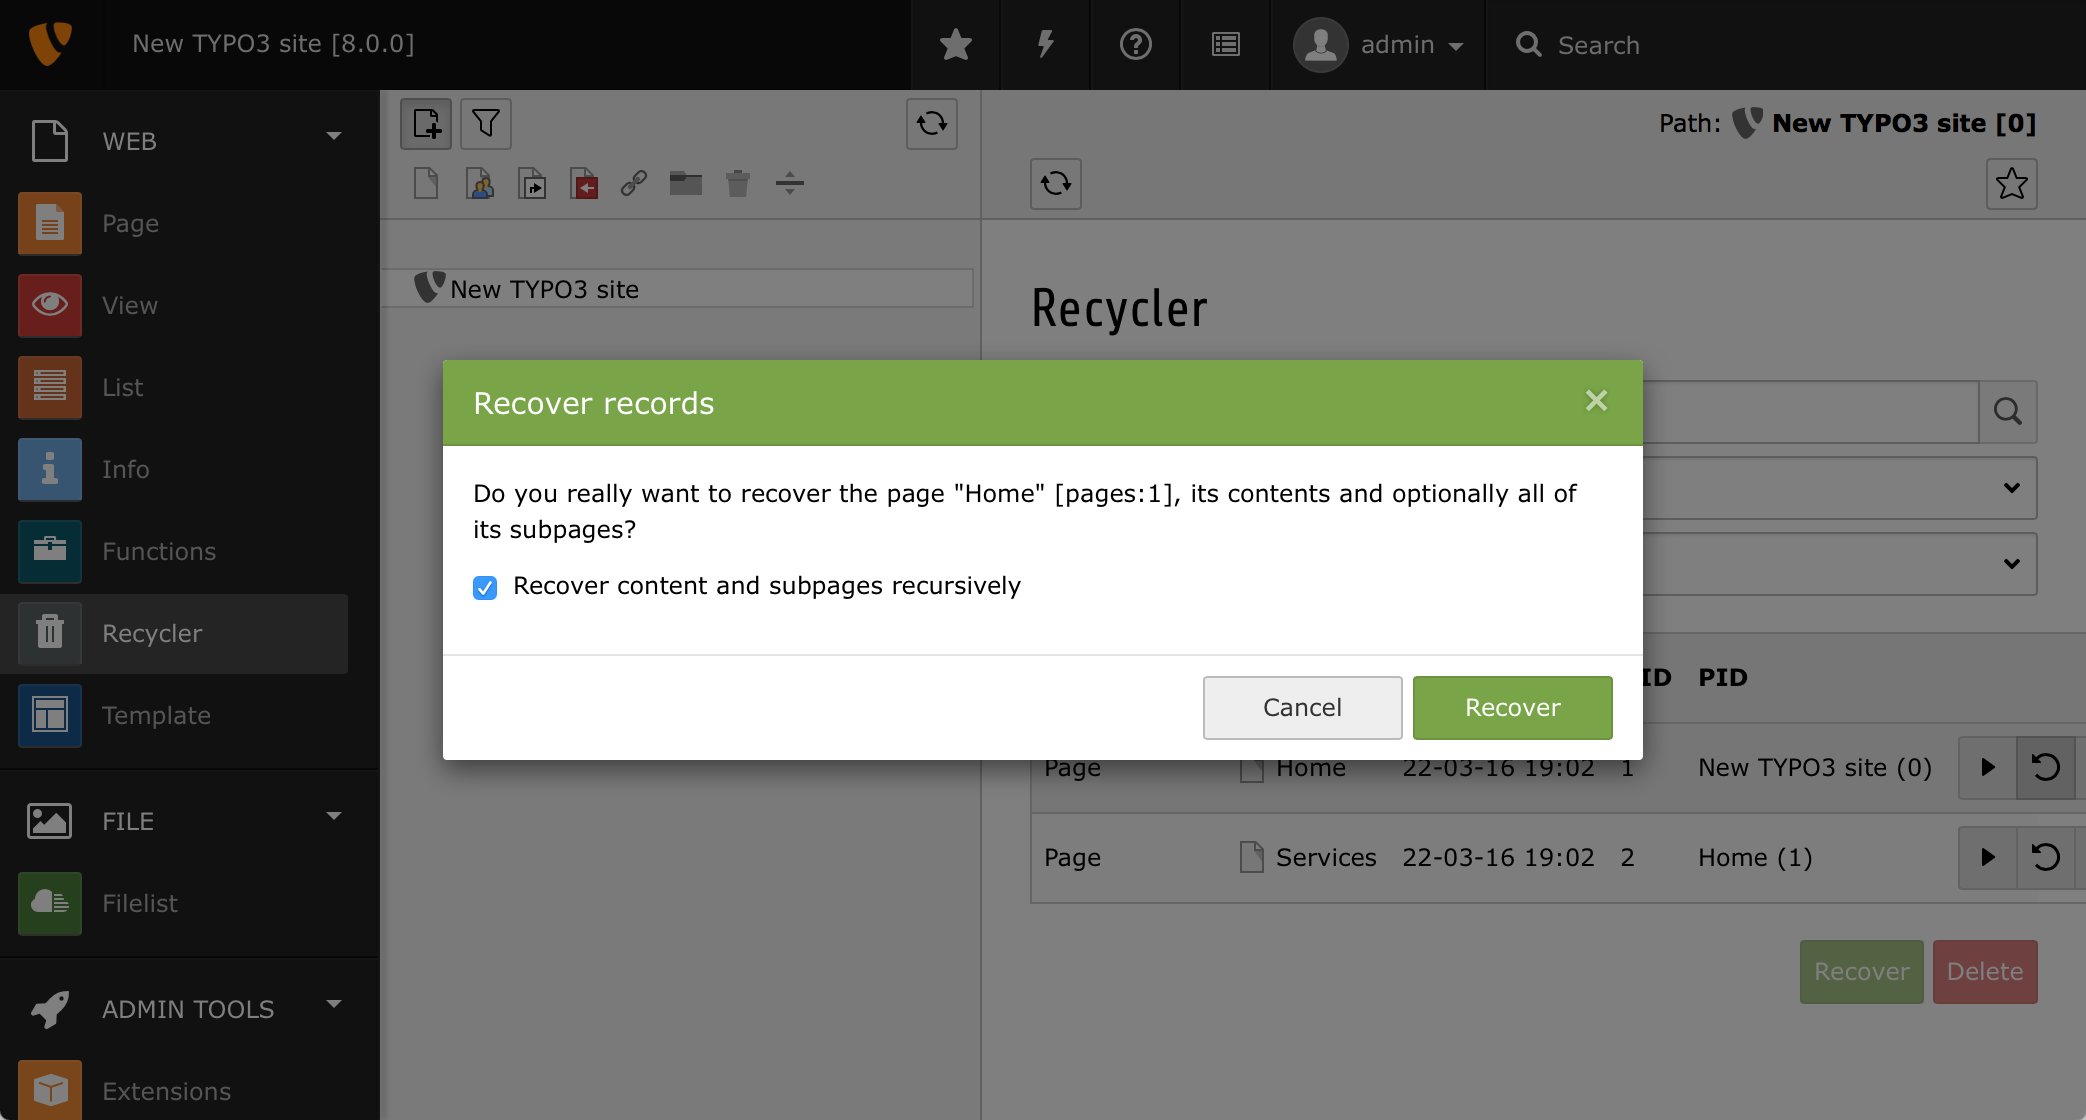
\includegraphics[width=0.70\linewidth]{BackendUserInterface/1835.png}
	\end{figure}

\end{frame}

% ------------------------------------------------------------------------------
% LTXE-SLIDE-START
% LTXE-SLIDE-UID:		8f6d7873-f5345466-084fd7ab-ad5b7fcf
% LTXE-SLIDE-ORIGIN:	04855567-dac16e24-f5274c64-f1d49c36 English
% LTXE-SLIDE-TITLE:		EXT:form - Directly load form wizard as inline wizard
% LTXE-SLIDE-REFERENCE:	!Feature-69394-EXTform-DirectlyLoadFormWizardAsInlineWizard.rst
% ------------------------------------------------------------------------------
\begin{frame}[fragile]
	\frametitle{Backend User Interface}
	\framesubtitle{Directly load form wizard as inline wizard}

	The wizard of EXT:form is loaded directly as inline wizard.
	There is no need to save and reload the newly created content element anymore
	in order to be able to open the wizard. This is a huge usability improvement.

	\begin{figure}
		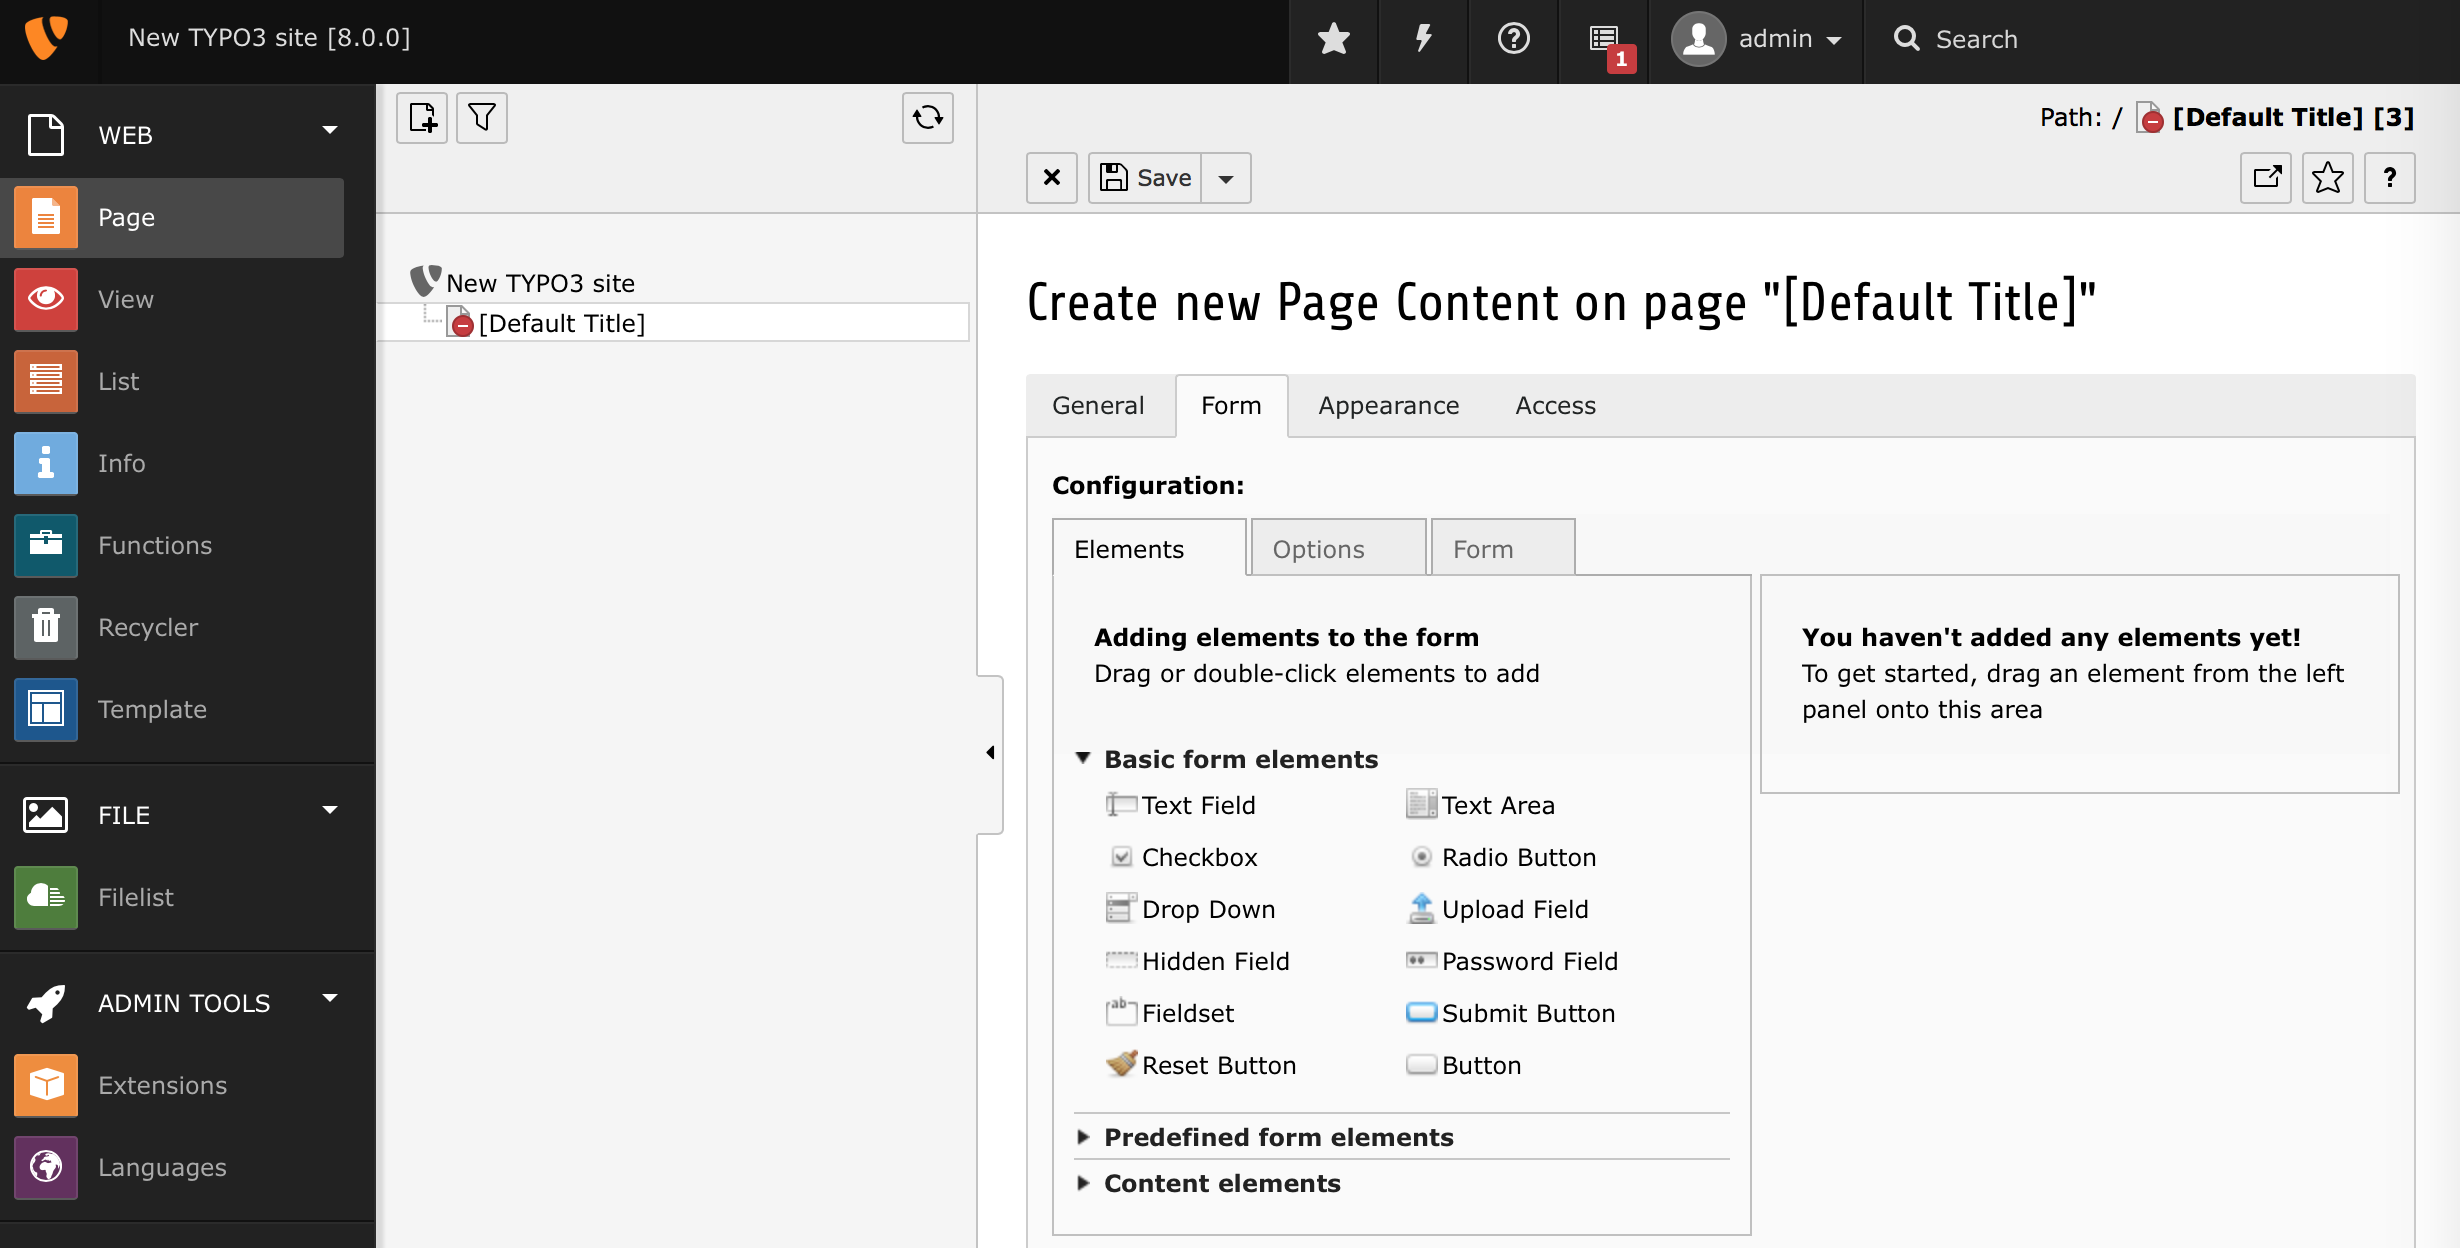
\includegraphics[width=0.70\linewidth]{BackendUserInterface/69394.png}
	\end{figure}

\end{frame}

% ------------------------------------------------------------------------------
% LTXE-SLIDE-START
% LTXE-SLIDE-UID:		c09d6c37-093fecff-5b765dbd-74e843d3
% LTXE-SLIDE-ORIGIN:	fd6d762a-b268caf0-cb6f9195-f553e035 English
% LTXE-SLIDE-TITLE:		Set the alternative backend logo via Extension Manager
% LTXE-SLIDE-REFERENCE:	!Feature-74109-SetTheAlternativeBackendLogoViaExtensionManager.rst
% ------------------------------------------------------------------------------
\begin{frame}[fragile]
	\frametitle{Backend User Interface}
	\framesubtitle{Set an alternative backend logo via Extension Manager}

	The backend logo in the upper left corner can now be configured in the extension configuration
	of EXT:backend in the Extension Manager.\newline
	Configuration options are:

	\begin{itemize}
		\item resource as a relative path of the TYPO3 installation\newline
			\smaller
				e.g. "\texttt{fileadmin/images/my-background.jpg}"
			\normalsize

		\item path to an extension\newline
			\smaller
				e.g. "\texttt{EXT:my\_theme/Resources/Public/Images/my-background.jpg}"
			\normalsize

		\item an external resource\newline
			\smaller
				e.g. "\texttt{//example.com/my-background.png}"
			\normalsize

	\end{itemize}

	\begin{figure}
		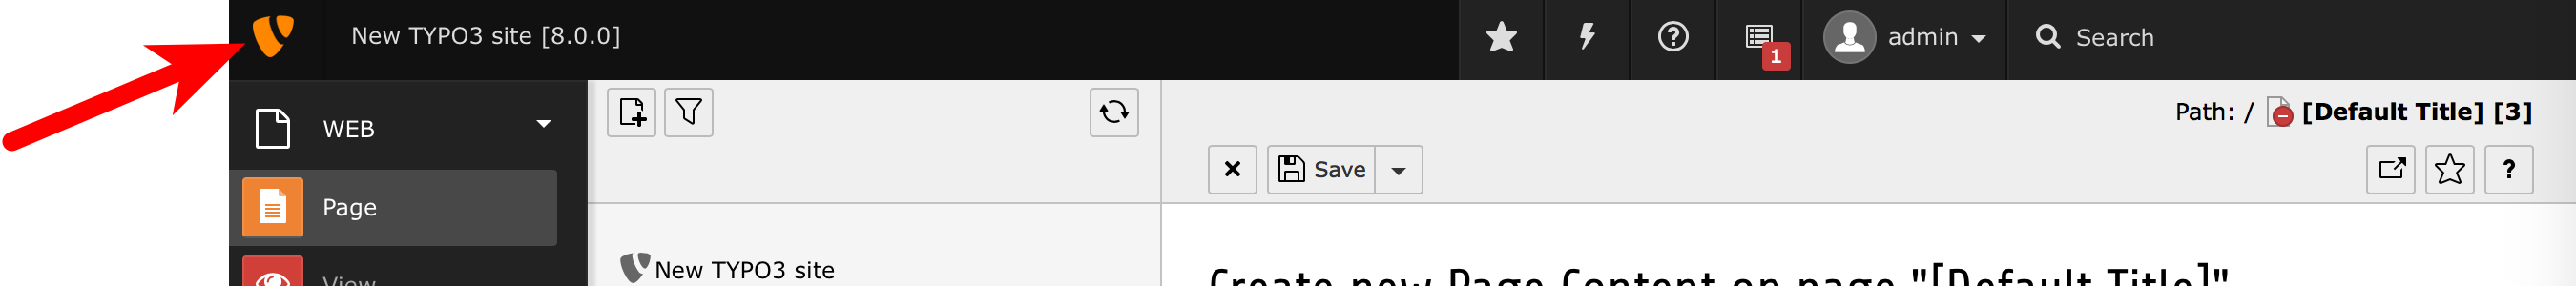
\includegraphics[width=0.7\linewidth]{BackendUserInterface/74109.png}
	\end{figure}

\end{frame}

% ------------------------------------------------------------------------------
% LTXE-SLIDE-START
% LTXE-SLIDE-UID:		37cc59ae-c5821747-37d4fa3f-2c52b49a
% LTXE-SLIDE-ORIGIN:	ab5ef36b-c670fbea-fd6d762a-cb6f9195 English
% LTXE-SLIDE-TITLE:		Page module: drag and drop supports copying now
% LTXE-SLIDE-REFERENCE:	!Feature-74179-PageModuleDragDropCanDoCopiesViaCTRLKeyNow.rst
% ------------------------------------------------------------------------------
\begin{frame}[fragile]
	\frametitle{Backend User Interface}
	\framesubtitle{Copy pages in drag \& drop mode}

	Additionally to the usual drag and drop feature in the page module (that \textit{moved} content elements),
	it is now possible to create copies: press the CTRL key while dropping to create a copy of the dragged
	element. After dropping is complete, the page module will reload to make sure the new element will be
	generated with all necessary information.

	\begin{figure}
		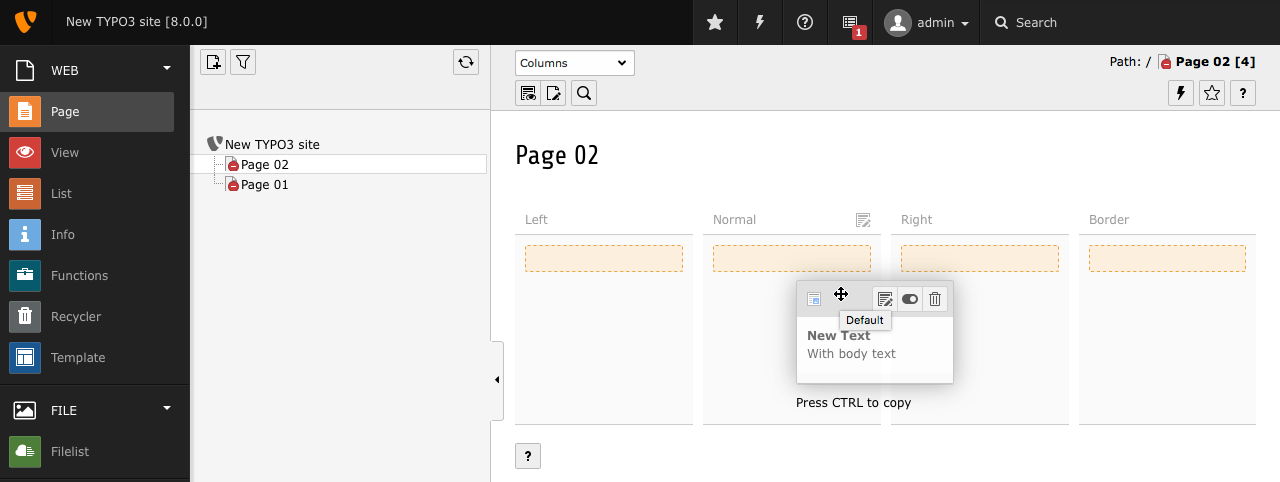
\includegraphics[width=0.7\linewidth]{BackendUserInterface/74179.png}
	\end{figure}

\end{frame}

% ------------------------------------------------------------------------------
